% Options for packages loaded elsewhere
\PassOptionsToPackage{unicode}{hyperref}
\PassOptionsToPackage{hyphens}{url}
%
\documentclass[
  openany]{book}
\usepackage{amsmath,amssymb}
\usepackage{lmodern}
\usepackage{setspace}
\usepackage{ifxetex,ifluatex}
\ifnum 0\ifxetex 1\fi\ifluatex 1\fi=0 % if pdftex
  \usepackage[T1]{fontenc}
  \usepackage[utf8]{inputenc}
  \usepackage{textcomp} % provide euro and other symbols
\else % if luatex or xetex
  \usepackage{unicode-math}
  \defaultfontfeatures{Scale=MatchLowercase}
  \defaultfontfeatures[\rmfamily]{Ligatures=TeX,Scale=1}
\fi
% Use upquote if available, for straight quotes in verbatim environments
\IfFileExists{upquote.sty}{\usepackage{upquote}}{}
\IfFileExists{microtype.sty}{% use microtype if available
  \usepackage[]{microtype}
  \UseMicrotypeSet[protrusion]{basicmath} % disable protrusion for tt fonts
}{}
\makeatletter
\@ifundefined{KOMAClassName}{% if non-KOMA class
  \IfFileExists{parskip.sty}{%
    \usepackage{parskip}
  }{% else
    \setlength{\parindent}{0pt}
    \setlength{\parskip}{6pt plus 2pt minus 1pt}}
}{% if KOMA class
  \KOMAoptions{parskip=half}}
\makeatother
\usepackage{xcolor}
\IfFileExists{xurl.sty}{\usepackage{xurl}}{} % add URL line breaks if available
\IfFileExists{bookmark.sty}{\usepackage{bookmark}}{\usepackage{hyperref}}
\hypersetup{
  pdftitle={Word embeddings for the analysis of ideology and identity in Canadian politics},
  pdfauthor={Justin Savoie},
  hidelinks,
  pdfcreator={LaTeX via pandoc}}
\urlstyle{same} % disable monospaced font for URLs
\usepackage{longtable,booktabs,array}
\usepackage{calc} % for calculating minipage widths
% Correct order of tables after \paragraph or \subparagraph
\usepackage{etoolbox}
\makeatletter
\patchcmd\longtable{\par}{\if@noskipsec\mbox{}\fi\par}{}{}
\makeatother
% Allow footnotes in longtable head/foot
\IfFileExists{footnotehyper.sty}{\usepackage{footnotehyper}}{\usepackage{footnote}}
\makesavenoteenv{longtable}
\usepackage{graphicx}
\makeatletter
\def\maxwidth{\ifdim\Gin@nat@width>\linewidth\linewidth\else\Gin@nat@width\fi}
\def\maxheight{\ifdim\Gin@nat@height>\textheight\textheight\else\Gin@nat@height\fi}
\makeatother
% Scale images if necessary, so that they will not overflow the page
% margins by default, and it is still possible to overwrite the defaults
% using explicit options in \includegraphics[width, height, ...]{}
\setkeys{Gin}{width=\maxwidth,height=\maxheight,keepaspectratio}
% Set default figure placement to htbp
\makeatletter
\def\fps@figure{htbp}
\makeatother
\setlength{\emergencystretch}{3em} % prevent overfull lines
\providecommand{\tightlist}{%
  \setlength{\itemsep}{0pt}\setlength{\parskip}{0pt}}
\setcounter{secnumdepth}{5}
\usepackage{booktabs}
\usepackage{amsthm}
\makeatletter
\def\thm@space@setup{%
  \thm@preskip=8pt plus 2pt minus 4pt
  \thm@postskip=\thm@preskip
}
\makeatother
\usepackage{float}
\usepackage[left=3cm,right=3cm,top=3cm,bottom=3cm]{geometry}
\usepackage{fontspec}
\usepackage{multirow}
\usepackage{multicol}
\usepackage{colortbl}
\usepackage{hhline}
\usepackage{longtable}
\usepackage{array}
\usepackage{hyperref}
\ifluatex
  \usepackage{selnolig}  % disable illegal ligatures
\fi
\usepackage[]{natbib}
\bibliographystyle{apalike}

\title{Word embeddings for the analysis of ideology and identity in Canadian politics}
\usepackage{etoolbox}
\makeatletter
\providecommand{\subtitle}[1]{% add subtitle to \maketitle
  \apptocmd{\@title}{\par {\large #1 \par}}{}{}
}
\makeatother
\subtitle{\hfill\break
Department of Political Science, University of Toronto\\
~\\
Dissertation Research Proposal}
\author{Justin Savoie}
\date{2021-09-15}

\begin{document}
\maketitle

{
\setcounter{tocdepth}{1}
\tableofcontents
}
\setstretch{1.75}
\hypertarget{intro}{%
\chapter{Introduction}\label{intro}}

Patterns of political beliefs are not random. People who hold certain ideas often hold others. An individual on the ``political left'' is likely to hold views clustering in certain specific ways with regards to, for instance, economic redistribution, immigration policy, environment policy, or human rights. Similarly, an individual on the ``political right'' will hold relatively coherent beliefs, and often different, to those held by a leftist. Of course, the political space is not perfectly unidimensional or bi-dimensional, or x-dimensional. Researchers and analysts often disagree about the number of dimensions, or the best ways to label them. At minimum, they usually agree it depends on context. For instance, introductory textbooks talk of a unidimensional left-right spectrum, or a bi-dimensional (Authority/Liberty--Left/Right) spectrum \citep{heywood2017political}. \citet{heroux2016substate} uses statistical modeling to identify five dimensions in the Canadian context. Neither do such clusters or dimensions possess universal or time-invariant validity. In the Canadian province of Québec, it is widely recognized that there has been a realignment, from a dominant federalism/sovereignty dimension to a more traditional left-right dimension \citep{montigny2016fin}. Nonetheless, there is a consensus that ``left'' and ``right'' are meaningful concepts when talking about politics, and that spatial representations of politics do help us make sense of the political landscape. One can make sense of ideology through some form of ``empirical reduction''.

Similarly, one can make sense of ``identity'' through similar techniques. Without a doubt, political identities are plural and wavering \citep[\citet{ozkirimli2017theories}]{hobsbawm2012invention}. Still they can be fruitfully studied to extract a core; to tell something about the identity's root \citep{schwartz1967public}. As the researcher can place the subject amid a spatial ideological representation, one can associate empirical symbols to cluster of political identities \citep{dufresne2019symbolic}.

One important way, and in a sense the only way, to study political beliefs (about ideology or identity) is through language; through what people say orally and in writing. All human communication requires language, words, and meanings. This is apparent in all approaches to the study of politics. It is most obvious in political theory, where commentators reflect at lengths over questions of politics, justice, or institutions, and in qualitative research, where analysts examine the deep structure of some data, usually linguistic in nature. Yet, in the social sciences, language also features centrally in quantitative work; most survey statistics uses linguistic data (questions, survey choices), ideal points models estimate ideology from roll-call data, i.e., data representing whether a politician agrees with specific policies or bills.

Traditionally, scholars have studied patterns of political beliefs (political ideology or political identity) either through quantitative approaches (surveys, scaling, scores of various natures, etc.) or through theoretical approaches (political theory, interpretative approaches, critical approaches, etc.) Of course, it has been common to combine these approaches; to combine thicker and thinner descriptions, as befits the object of study.

Automatic content analysis methods have long promised to try to bridge the gap between quantitative and qualitative-theoretical perspectives. It has been difficult: extracting meaning from text is hard. It is not for lack of effort: political scientists have laboured intensively on text scaling methods. Approaches based on word frequencies in text \citep[\citet{laver2003extracting}]{slapin2008scaling} allow to compare policy positions. Supervised classification of political texts into known categories help us study tone, partisan affiliation, or any pre-determined categories which an algorithm can learn and then put texts into. These methods have allowed us to make important advances. Nevertheless, they remain at a high level of abstraction. The unit of analysis is the document in the case of text scaling; classification is useful but does not really get at the sense or the meaning in the text.

Word embeddings have recently emerged as a promising way to get at meaning. Word embeddings stem from statistical semantics and can be summarize by the distributional hypothesis: words used and occurring in similar contexts tend to have similar meanings. It is then possible to model and represent in high dimensional space each word (or each political concepts if they are represented by one or several words). Technical advances (the idea behind word embeddings has been around for decades but efficient and mainstream implementation is recent \citep[\citet{mikolov2013efficient}]{mikolov2013distributed} have the potential to offer new perspectives to the study of political meaning. Some researchers have started using such methods, but, in the social sciences, their use is still in its infancy. My dissertation uses statistical semantics to study ideology and political identity in Canada. Using textual data from transcripts of Parliamentary Debates (1900-2019) and Twitter data, I study patterns of word use, over time and context (e.g.~elites vs non-elites, left vs right). I aim to get at word and concept meaning, using word vectors, in the context of discussions about Canadian politics.

\hypertarget{research-questions}{%
\chapter{Research questions}\label{research-questions}}

The main research question in this study is: can we use word embeddings to document and map the changing meaning of key terms used when talking about politics in Canada? Is it possible to reproduce, even in an approximate form, a `commonly-accepted-among-scholars' analysis of the development of the meaning of four key concepts in Canadian politics: rights, identity, citizenship, and nation. Such an approach combines the scope of conceptual approaches with at least some of the breadth of linguistic approaches, while capitalizing on quantitative method's empirical grounding. I define ideology and identity in a broad sense as the thoughts, beliefs, attitudes, behaviours, and values that are related to politics.

\hypertarget{literature-review}{%
\chapter{Literature review}\label{literature-review}}

\hypertarget{from-quantitative-large-n-surveys-to-word-embeddings}{%
\section{From quantitative large-N surveys to word embeddings}\label{from-quantitative-large-n-surveys-to-word-embeddings}}

People holding certain political beliefs often hold others. In this dissertation, I call ideological analysis the general study of those political beliefs. Ideological analysis, in this context, includes the study of what empirical political science usually calls ideology (latent policy dimension), but also symbols and markers of political identity. Ideology, thus understood, is a loaded term; it can mean very different things. These meanings range from the French ideologues's ``objective'' study of ideas just before and during the French revolution \citep{kennedy1979ideology, head1985ideology} to illusion, mystification or false consciousness in Marx and Engels' German Ideology \citeyearpar{marx1970german}, or a morphological, conceptual, non-pejorative map of the sociopolitical world \citep{freeden2003ideology}, and include various spatial scaling methods; measuring what is called the left and right, conservative and liberal positions; in one, or multiple dimensions; measurable in real life \citep{downs1957economic, aldrich1977method, hare2015using, cochrane2015left} or online \citep{barbera2015birds, temporao2018ideological}. Understanding precisely the patterns that hold these ideas together is a matter of considerable debate. \citet{maynard2013map} divides in three broad groups these motley vantage points: conceptual approaches, discursive approaches and quantitative approaches.

Conceptual approaches focus on systems of ideas: concepts and their complex interrelations function as the unit of analysis. Ideologies provide frameworks from which individuals understand the world. Freeden's \citeyearpar{freeden2006ideology} morphological approach is an influential example. Foundational principles such as ``liberty'', ``security'' or ``equality'' are shared by the great vast majority, yet adherents of different ideologies understand those principles in a different and sometimes conflicting way. Political concepts acquire meaning through discourse, culture and positionality. Ideologies evolve through conceptual competition; through ``decontestation''. Other scholars working in this tradition include Reinhart Koselleck (conceptual history), and Quentin Skinner (Cambridge School of historicist and contextualist interpretation). Some have formalized this analysis of the structures that underlie social interactions, via, for instance, complex systems \citep{thagard2012mapping, homer2014conceptual}.

Discursive approaches focus on communicative practices. They are less concerned with content, and more concerned with visibility, power, and influence. Crucially, they usually involve a critique of ideology from the left. While epistemological disagreement exists on matters of relations to truth, with post-structural discursive approaches \citep{mouffe1985hegemony, zivzek1989sublime} more sceptical than critical discourse approaches \citep{van2006ideology, fairclough1992discourse}, both strands share a commitment to the critique of naïve conceptions of truth \citep{kellner1989critical}. Vast methodological differences also cleave the field, from the study of semantics \citep{pecheux1975language}, to the post-Marxist attention paid allegory \citep{jameson2020allegory}, speed \citep{baudrillard1994simulacra} , spectacle \citep{debord2012society}, or empty signifiers \citep{laclau2007emancipation}. Through the study of linguistics or discursive constructions, critical approaches hence shed light on the origins of, and the process by which, ideas, which may or may not be, but usually are, problematic and alienating, come to reproduce themselves to the point of insidious symbolic hegemony. Recently, discursive analysis has been extended to include statistical based approaches \citep{nafstad2012ideology} relying largely on word count. In the context of ideological analysis, frequency usage of communality words (solidarity, welfare) or words linked to consumerism can provide insight in possible changes in the way individuals construe and reproduce political behaviours \citep{nafstad2012ideology}.

Quantitative approaches use large-N analyses to study patterns of beliefs. A divide exists between observational studies of ideology studying citizens' stated preferences \citep{bonica2013ideology} or legislators' voting behaviour \citep{martin2002dynamic}, and approaches in social psychology, rather focusing on cognitive biases, links between belief systems and personality; ideology as social cognition, for instance by linking political preferences to psychological inclinations toward uncertainty or threat \citep{jost2013political}. Quantitative approaches also include traditional dimensionality reduction, where values are reduced to dimensions: see \citet{heroux2016substate} for an investigation of the Canadian case; \citet{cochrane2010left} for a study of ideological asymmetries.

As such, ideological analysis is fragmented. For instance, experimental social psychology can look down on non-experimental approaches, where falsification is less straightforward. Conversely, non-quantitative scholars can look down upon the poor external validity of experiments, or their theoretical levity. Calls have been made to see, use and combine the full variety of available approaches. Especially, to see ideological analysis as ``a field in its own right'': researchers from various strands have common core objectives, how people talk about politics, and how it is significant \citep{maynard2013map}.

My dissertation proposes such a combination of frameworks to study ideology. Substantively, I aim to map the changing meaning of political words over ideology, time and ideology/time interactively. Methodologically, I will call upon recent advances in the computer science field of natural language processing. Namely, the dissertation's methodological workhorse will be word embeddings: a set of techniques where words, phrases or documents are mapped to vectors of numbers. Conceptually, word embeddings organize words, phrases or documents in high dimensional space, where similar items are close to each other and dissimilar items are not. Perhaps, `immigrant' will be close to `refugee' but not to `parliament'; `parliament' will be close to `institution', but not to `climate change'. Embeddings are calculated based on distributions of words in large corpora, and their proximity to other words. In other words, in linguist J.R. Firth's \citeyearpar{firth1957papers} now celebrated terms: ``You shall know a word by the company it keeps''.

Most work in the quantitative social sciences has studied ideology from the point of view of dimensionality reduction and regression. Dimensionality reduction is ambiguous in what it reveals. Dimensionality reduction tells us if there is a fit between political beliefs \citep{gregg1965dimensions}, but not how it forms or where it's from. Regression analysis finds bivariate or multivariate links. For instance, in average, education is related to views on abortion. Neither approaches are perfect as they often fail to explain family resemblance-like phenomena. Left-right positioning is one such phenomena \citep{cochrane2015left}. It arises when it's not that members of a family have significantly bigger noses, or lighter-eyes, or darker hair than the rest of the population. Rather, it's when some combination of those characteristics makes it likely to hold others. In politics, such combinations are frequent. Studying the emergence of fringe communities and political echo chambers using closeness centrality in a network can reveal multiple communities and their interactions in a way impossible to traditional statistical methods \citep{boutyline2017social}. Ideological scaling and spatial models of politics using traditional statistical methods or network approaches then allow to address one of the most salient questions for academics and citizens alike: to what extent is society ideologically polarized, and is there increasing polarization?

Work on ideology and spatial representation has mostly used likert-type items. Dimensionality reduction is often used on categorical, ordinal or numerical variables. This way of working limits possible nuance for the respondent but simplifies the researcher's task. Working on a set of questions with answers varying only over a certain range or a certain support entails postulating that the ideological world can be conceptualized as such. Yet, making this chief assumption allows for useful and enlightening insight on the structure of politics (for a classic example see \citet{aldrich1977method}). It certainly would involve some work, but it appears reasonable to believe that replacing close-ended question by longer open-text when studying political ideology, would allow to extract more substance, and increase the precision of our ideological model \citep{bauer2017left}.

Recent work has focused on exactly this: fitting models predicting the use of words in context to generate estimates of ideological placement \citep{rheault2020word, rodman2020timely}. Thus, I propose to extend such work. These models often use word embeddings \citep{rumelhart1986learning, mikolov2013efficient, mikolov2013distributed}. Each word is mapped to a large numerical vector. The given vector represents the context in which the word is generally used. The method depart significantly from bag-of-words methods traditionally used in political science where word count is the main predictor of various outcome measures. \citet{rheault2020word} have argued that taking into account the role of words in context is especially promising for scholars attempting to measure political ideology. Patterns of ideas often are tangible, but irreducible as ideology functions in a network-like way: ideas are loosely associated, clusters or patterns emerge, people know ideology when they see it, yet struggle to name things as they are. Ideology functions in a plastic way. \citep{cochrane2015left} Word embeddings, since words are at the center of the network of words with which they are used, are designed to capture such interplay.

Usually, researcher study only one single type of texts. \citet{rheault2020word} study parliamentary texts. \citet{rodman2020timely} analyses newspaper articles from the New York Times, Reuters and Associated Press. \citet{rodriguez2021word} model words in congressional speeches. This dissertation aims to model word use and ideology from various sources: citizens, journalists, and parliamentary text. Political ideology does not arise from debates in parliament only. Similarly, pundits or political theorists do not have the monopoly over the way language is used to express political belief. Ideology emerges not within one social group or institution, but through social practices shared by citizens, politicians, pundits, theorists alike. There will be some differences, but a language-based theory of ideology must be applicable to more than one case. The study of ideology should be pluralistic in its objects: various actors, from all over society, produce ideological speech, in turn influencing the speech of various actors.

One common difficulty arising from the modelling of ideology through text motivates this research. Often, such modelling identifies other dimensions, clearly non-ideological \citep{hirst2010party, lauderdale2016measuring}. Instead of capturing ideology, statistical models use words to learn ``something else'', like expressions of attack and defence, opposition and government, geographical differences, linguistic complexity, and so forth. Such findings emerge mostly from studies using word-count-like features, not word embeddings. Rheault and Cochrane's findings suggest embeddings might be a solution to this problem of ideological identifiability. The dissertation aims to test this solution on text non-parliamentary texts, and in more than one language.

One further difficulty concerns the measure of uncertainty. Producing estimates without measuring uncertainty can be misleading. Estimates without a measure of uncertainty can suggest a precise result that should actually be interpreted quite differently if a large uncertainty measure was reported. \citet{han2018conditional} propose a variational Bayesian approach for estimating parameter uncertainty. Several approaches to get at uncertainty can be tested. A first is to leverage the fact that embeddings are usually underdetermined. This means that running the same model twice gives different results. The numerical estimates will not be the same. However, if the model is successful, the relative results will be the same, i.e.~word will have the same ``meaning'' as measure through distance. Hence, one might be able to measure uncertainty through some form of bootstrapping The second method would be similar, also using bootstrapping but with replacement, changing the text slightly each time; but replacing words with similar words. Estimates with uncertainty will be measured against ``objective measure of ideology''. In the case of citizens, this can take the form of vote choice, or self-placement on a numerical axis. For pundits or politicians, it can be more complicated to find an objective measure. Comparing estimates and their uncertainty to expert judgments, the idea is to produce estimates that generally make sense. For example, measuring the ideology of politicians in the Canadian parliament, members of the New Democrat Party should be to the left, members of the Liberal Party of Canada in the center, and members of the conservative party on the right, uncertainty should overlap between and within parties.

\hypertarget{distributional-semantics}{%
\section{Distributional semantics}\label{distributional-semantics}}

The previous subsection has introduced the idea of word embeddings: high dimensional vectors encoding the meaning of a word such that similar words have similar positions; are close to one another. In that section, word embeddings have been presented as one interesting way to produce some empirical ideological analysis; as the latest in a series of quantitative methods to study political behaviours and ideas. The present section shifts the focus on the linguistic properties and foundations of word embeddings: word embeddings as part of the research area called distributional semantics, or distributional approaches generally. Many of the ideas explored are largely inspired by \citet{sahlgren2008distributional}.

Sahlgren suggests distributional approaches rely on a set of assumption referred as the ``distributional hypothesis''. This hypothesis can be stated in various forms:

``words which are similar in meaning occur in similar contexts'' \citep{rubenstein1965contextual}; ``words with similar meaning will occur with similar neighbors if enough text material is available'' \citep{schutze1995information}; ``a representation that captures much of how words are used in natural context will capture much of what we mean by meaning'' \citep{landauer1997solution}; and ``words that occur in the same contexts tend to have similar meanings'' \citep{pantel2005inducing}.

Sahlgren summarises: the distributional hypothesis is about ``a correlation between distributional similarity and meaning similarity which allows us to utilize the former in order to estimate the latter''.

To examine this ``distributional hypothesis assumption'', two questions can be asked. The first question is about the kind of distributional properties we are looking for (and in practice a question about algorithms). The second question asks ``in what sense it is meaning that is conveyed by distributional patterns'' \citep{sahlgren2008distributional}. The first question, about the choice of algorithm, will be covered in the next section on methodology. What it means to get at meaning through word embeddings is explored in this section. This will be expanded in the dissertation.

The key idea discussed will be the common critique raised against distributional semantics and word embeddings: that they do not get at meaning because they only study the text, and not the world. Sahlgren's narrative is about the structuralist foundations of distributional approaches. Theories of meaning often ask if meaning is to be found in the mind (e.g.~idealism), in the world (e.g.~materialism, physicalism) or in the text (e.g.~structuralism word embeddings). A model of meaning can situate it in anyone of mind, world or text, but situating it in the text has the pragmatic advantage of predictive power and of current large scale use. Work in political science usually mentions Firth and the distributional hypothesis \citep{rheault2020word, rodman2020timely, rodriguez2021word, rodriguez2021embedding} but, usually stops at Firth. The point of this grounding in structuralism is that it makes explicit what can be shown with word embeddings and what cannot (i.e.~word embeddings are not very useful from the perspective of a Correspondence Theory of Truth or a Verificationist Theory of Truth, but useful from the perspective of a Pragmatist or Coherentist theory of Truth; they make sense if you accept meaning holism and they don't if you swear by atomism about meaning). It is not necessarily evident why such a discussion belongs in political science, rather than in philosophy, but I think it is useful to reply to one frequent objection to text-as-data methods: that they don't work in practice. I think that sometimes they work well and sometimes they don't, but that mostly they are useful. In particular, I think that discussing some arguments in favor and against meaning holism can help alleviate problems associated with the intuition that words should have one-to-one relations with objects outside of the text.

\hypertarget{ideology-and-identity-in-canada-changing-meanings}{%
\section{Ideology and identity in Canada: changing meanings}\label{ideology-and-identity-in-canada-changing-meanings}}

This theoretical and methodological setup is necessary although secondary to the main objective: describing and measuring the changing meanings of key concepts used to talk about Canadian politics. Canada has a different history than those countries we usually think of as most similar, namely the United States and countries in Western Europe. Living next to the U.S. is like ``sleeping with an elephant'' said Pierre Trudeau, at the same time its European origins remain evident \citep{resnick2020european}. Canada's identity has always been ambivalent, is it mono-national or pluri-national, does it have a culture, a ``biculture'', or ``multicultures''; what about aboriginal cultures? \citep{wiseman2011search} And, of course, is this changing, and how, over time? To cite a recent paper, describing this ambivalence \citep{dufresne2019symbolic}:

\begin{quote}
``In a nutshell, Canada is an immigrant nation founded, quite recently, on native land over an enormous territory by two linguistically distinct colonial groups -- the English and French. If we add to this a hegemonic threat from a powerful American neighbour, a Quebec separatist movement, strong regional resentment in the West, and Aboriginal claims, Canada's difficulty in finding shared symbols to define the nation seems unsurprising.''
\end{quote}

Studying Canadian ideology and identity, we will focus on what it means to be Canadian. The question will be addressed both from the angle of identity (what it means culturally, origins, symbols) and ideology (does citizenship ``involves'' redistribution, openness to immigrants, justice, etc.). We identify four key concepts: citizenship, identity, nation and rights. A more extensive literature review will be included in the dissertation. For now, we can say that Canadian identity and nationhood was intrinsically linked to a ``British connection'' for close to 100 years following Canada's founding in 1867. This ``British connection'' of course was not part of the identity of those identifying as French Canadians. Starting in the 1960s, following similar developments in other Western countries, a diversification of identity claims began. In many ways, being Canadian was not necessarily about being French, English/British or Indigenous, but from a more plural and heterogeneous experience, some would say a post-national experience. Around the same time, Canada experienced a constitutional maturation with a Rights Revolution. Between 1931's Statute of Westminster, when Canada achieved independence from Britain and 1982's patriation when Canada obtained full sovereignty over it's constitution, there was the emergence of a ``rights mentality'': individual rights were becoming less abstract, and more something that Canadians could rely on in their day to day lives.

Where were politicians in the House of Commons standing on these developments? Empirically, around what period can we start to see a decline of ``Britishness talks''? Similarly, can we observe the rise of ``rights talk''? These questions are explored in the chapter on semantic change in the House of Commons.

\hypertarget{methodology}{%
\chapter{Methodology}\label{methodology}}

The use of word embeddings in social scientific research is relatively recent. \citet{kozlowski2019geometry} are the first to use them to analyze the meaning of words in social discourse, producing a cultural analysis of discourse in a major social science journal. In political science, \citet{rodman2020timely} is the first to produce a thorough analysis of the use of diachronic embeddings to study semantic change. \citet{rheault2020word} use word embeddings to study political discourse, but their focus in on ideological placement rather than on the use of embeddings for semantics or sematic change. Recent work also provides guidelines to the applied researcher. \citet{rodriguez2021word} focus on general guidelines to train embeddings efficiently: algorithms, parameters, pre-trained vs newly trained embeddings, etc. Their focus is on the general machinery of word embeddings rather than on semantic measurement per se. In another methodological paper, \citet{rodriguez2021embedding} focus on semantic change across groups in time. Their method, called à la Carte on Text (conText), extends a linear model, through multivariate regression, refitting pre-trained embeddings to local contexts. One objective of this methodological chapter is to present possible approaches to measuring how a word's meaning varies over circumstances; over time or other covariates. Five models in particular will be tested, the first four first presented by \citet{rodman2020timely}, the fifth presented in \citet{rodriguez2021embedding}: (1) naïve time series, (2) overlapping model (3) aligned model (4) chronologically trained model (5) à la Carte on Text. This chapter does not present any new results, it rather presents in detail methods used to produce embeddings in social science. An overview is presented in this proposal; more technical details will be given in the dissertation.

\hypertarget{word-embeddings}{%
\section{Word embeddings}\label{word-embeddings}}

Using word embeddings, each word from a given text is mapped to a large numerical vector. The vector's dimension is determined by the researcher; usually between 100 and 500 \citet{rodman2020timely}. The given vector represents the context in which the word is generally used. The model can be trained by predicting the word with its context, i.e.~the other words around it, on a given window; this is the CBOW model. Alternatively, one can predict the context with the word using the skip-gram model. The GloVe method similarly models word and their context. The main difference is that it takes into account explicitly a matrix of co-occurrences. That is, word frequency enters in the modelling. In practice, these methods are similar, it is not entirely clear when and why they perform better, and GloVe is generally the preferred option in social science \citet{rodriguez2021word}. Yet, in general, one of the most popular implementations is through the well-known gensim Python library. As a default, gensim uses CBOW. For instance, the two most recent use of word embeddings in political science use gensim \citep[\citet{rheault2020word}]{rodman2020timely}.

\hypertarget{doc2vec}{%
\section{doc2vec}\label{doc2vec}}

There exists an extension to word2vec called doc2vec which embeds paragraphs or documents in the same vector space as words. The paragraph or the document can be thought of as an extra word; and items can be compared. Doc2vec is particularly useful to map the ideological position of a politician or a citizen in this vector space. An example of logical result would be that conservative politician's embedding will represent a point in space closer to words about the economy or a traditional lifestyle, while a liberal or progressive politician will be mapped to a point closer to words about social justice or redistribution.

\begin{figure}
\centering
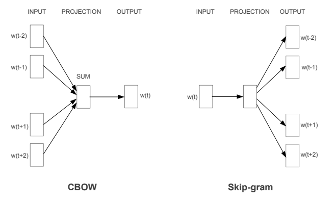
\includegraphics{figures/methodology-cbow-skipgram.png}
\caption{\label{fig:unnamed-chunk-2}Continuous Bag of Words and Skip-gram architectures}
\end{figure}

\hypertarget{diachronic-embeddings-and-semantic-change}{%
\section{Diachronic embeddings and semantic change}\label{diachronic-embeddings-and-semantic-change}}

Measuring changing meaning implies that different words embeddings are calculated at different moments in time. In essence, this is what \citet{rodman2020timely} does. In her paper, she raises several issues. First, naturally, cut points will be arbitrary. This might or might not make sense. For instance, changing meaning on equality during the twentieth century might be a gradual process, but changing meaning on terror politics might be dramatic around events like September 11, 2011 or October 29, 1929. Arbitrary cut points therefore require careful thinking. Second, language often is polysemic or includes homonymies. For instance, ``black'' might be political in some contexts, and only about a color in others. Producing valid embeddings must take this into account. Third, and most importantly, there is the issue of non-comparability between models. Models position words in vector space. Distance can be calculated between words or documents. However, when looking at change in meaning over time, distances from words in many models are compared. This can be a problem as words across models are not aligned \citep{hamilton2016diachronic}. Rodman provides the analogy to factor analysis. When ran on multiple datasets, it is likely that dimensions produced by factor analysis are similar, yet, factor order might change, or loadings might be on scales which are, in the absolute, non-comparable. For these reasons, while measuring changing word meaning over time, the analyst must proceed with caution.

Several methods exist to deal with non-comparability. Rodman identifies four. A naïve model, where the non-comparability problem is ignored, an overlapping time series models where differences are smoothed across time by including some text from the previous period, a chronologically trained where the model is initialized using results from the previous period and aligned time series where naïve models are ran, then aligned using a matrix alignment. Rodman's work suggests that a chronologically trained model is the best. The dissertation will validate these assumptions on new datasets.

Other methods exist to deal with semantic change. Long Short Term Memory units (LSTMs) on word embeddings corresponding to time-periods \citep{boukhaled2019modelling}. Contextualized word embeddings like BERT and ELMo can also model diachronic semantic change \citep{kutuzov2020distributional}. These methods are more complex to implement and yet to be really used in the social sciences. I will say a few words about them but they will not focus centrally in this dissertation.

\hypertarget{uncertainty}{%
\section{Uncertainty}\label{uncertainty}}

Measuring uncertainty when using word embeddings is non-trivial. Yet, when social science researcher make inference, they must accompany with uncertainty statements. The methodology section will discussion the question of uncertainty. The focus will be on bootstrapping methods \citep{rodman2020timely} and bayesian methods \citep{han2018conditional, lauretig2019identification}

\hypertarget{capturing-the-dynamic-meanings-of-political-keywords-in-the-canadian-house-of-commons}{%
\chapter{Capturing the dynamic meanings of political keywords in the Canadian House of Commons}\label{capturing-the-dynamic-meanings-of-political-keywords-in-the-canadian-house-of-commons}}

Can we trace the changing meaning of keywords used to talk about politics? Using data from the Canadian Parliamentary debates dataset (Hansard) we model the changing meaning of the words `nation', `rights', `citizenship' and `identity'. This choice of words is only preliminary, the list will likely be expanded.

\citet{rodman2020timely} traces the meaning of the word equality in America between 1855 and 2016. In a first step, she uses embeddings to document the underlying structure of equality by asking: equality of what? With word embeddings, she shows how equality is discussed alongside race, gender, international relations and German affairs (for news related to World War II). We will provide a similar analysis for `nation', `rights', `citizenship' and `identity', in the Canadian context.

A working hypothesis is that prior to 1982 discussions of rights were less formal and more abstract, while after 1982, they were grounded in concrete examples. Similarly, debates on identity at the beginning of the twentieth century would have been centered on language, bilingualism or biculturalism, and only in recent years have moded to issues, of sex and gender, sexual minorities, race and multiculturalism. Recent work (Rheault and Cochrane, 2020) has shown that word embeddings and party embeddings can capture a latent concept like ideology. The chapter tests whether it is possible to measure the evolving meaning of concepts central in the history of Canadian politics. Two examples can help illustrate.

\begin{figure}
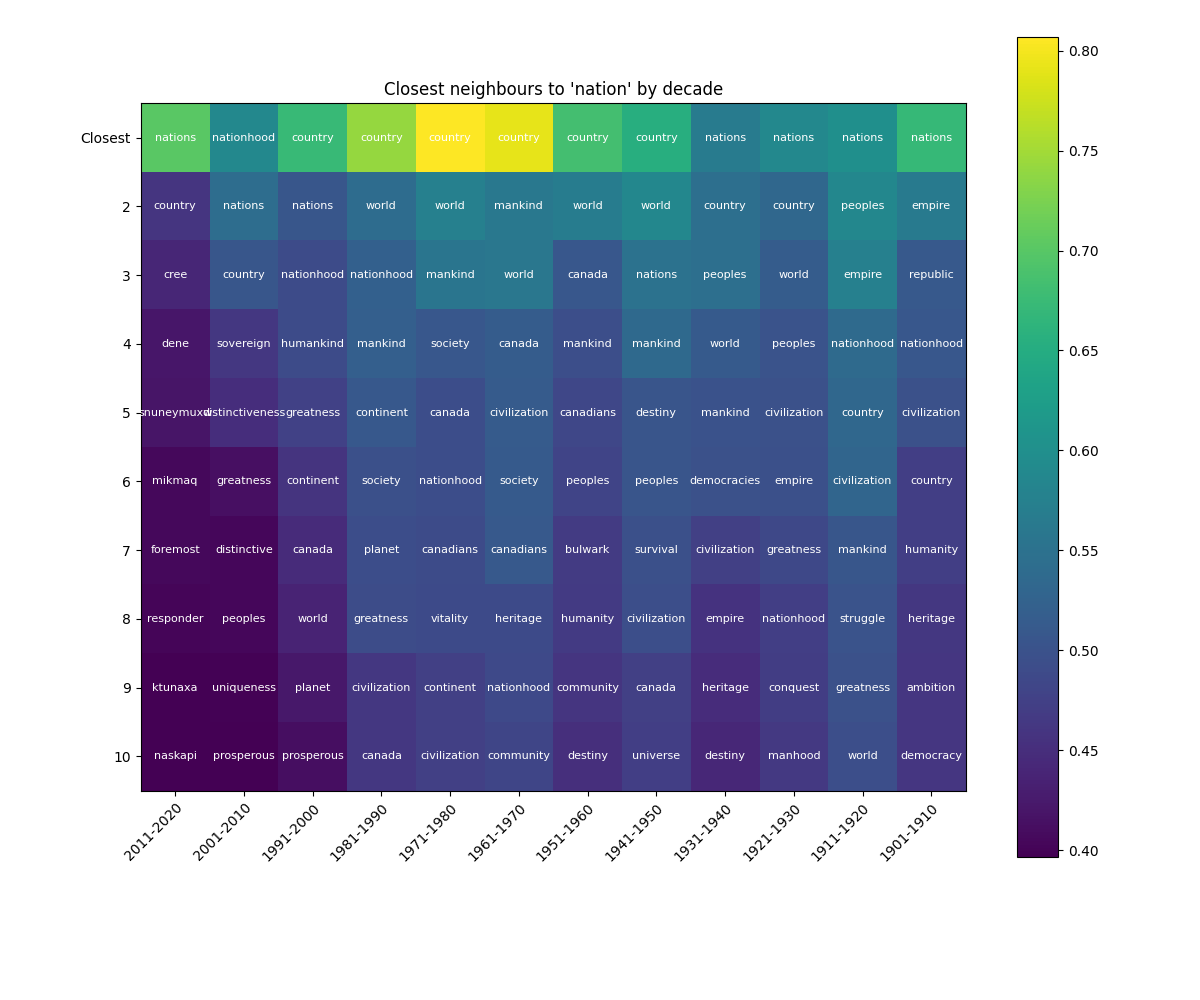
\includegraphics[width=1\linewidth]{figures/nation} \caption{Co-sine similarity to 'nation' by decade}\label{fig:unnamed-chunk-3}
\end{figure}

We use model data from the Hansard dataset to calculate a set of embeddings for each decade during the period 1901-2020. The model use is the default gensim implementation of CBOW with dimensions 300, window 6, using 15 iterations. This is equivalent to Rodman's ``naïve model''. Even with this simple specification, interesting results stand out. Figure 2 shows that during the first decade of the twentieth century, the closest words to `nation' using co-sine similarity were `nations', `empire', `republic', `nationhood' and `civilization'. By contrast during the most recent decade, the closest words to `nation' were `nations', `country', `cree', `dene' and `snuneymuxw'. During this most recent decade, six out of the 10 closest words to `nation' were Indigenous nations. It is the first decade that at least one Indigenous related word appears. As we can see, words such as `empire', `struggle', `conquest' or `survival' are semantically close to `nation' in early decades, but not in recent decades.

\begin{figure}
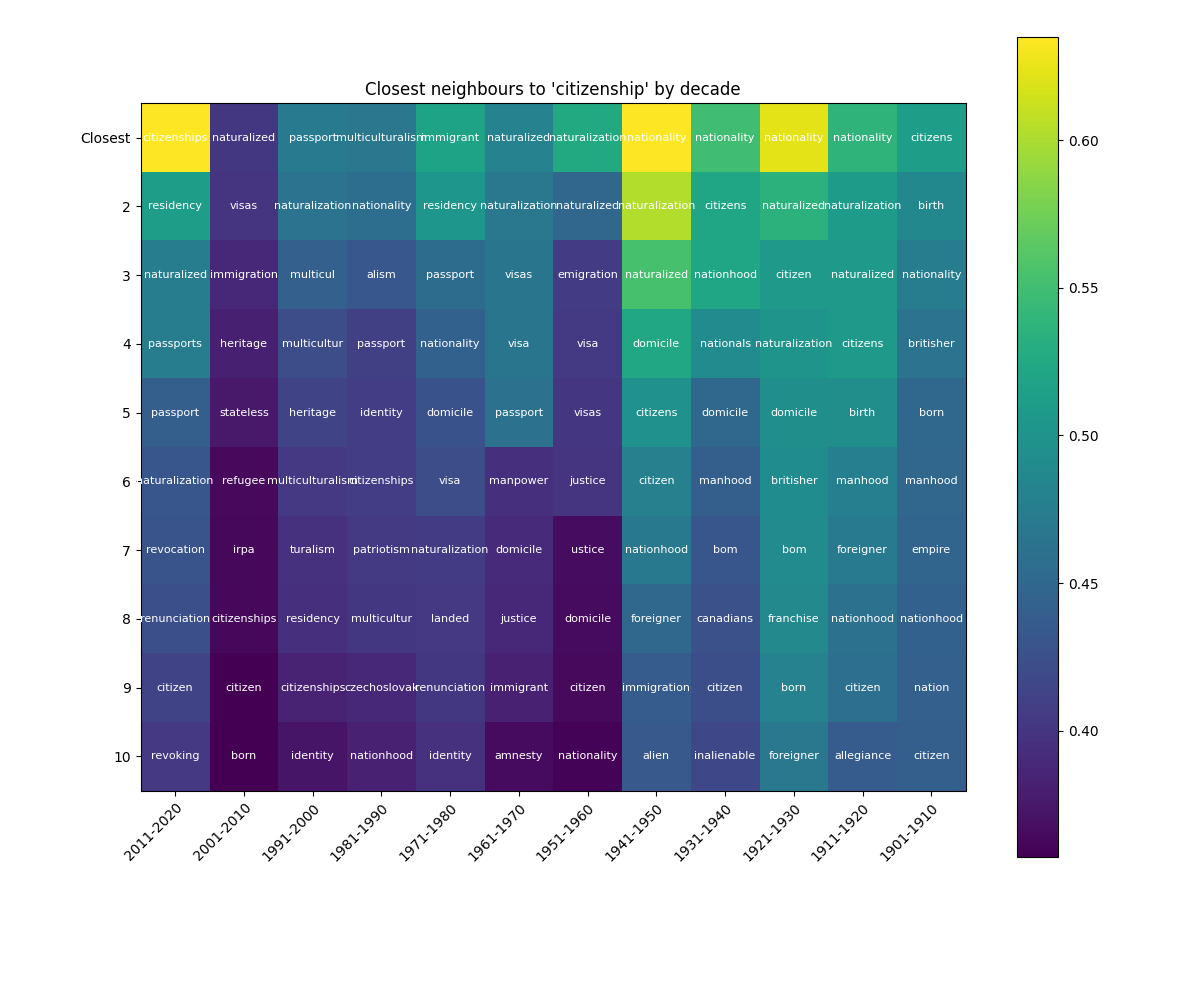
\includegraphics[width=1\linewidth]{figures/citizenship} \caption{Co-sine similarity to 'citizenship' by decade}\label{fig:unnamed-chunk-4}
\end{figure}

Figure 3 shows results that parallel those just discussed. Using the same word embeddings model, we visualize the closest neighbours to `citizenship' by decade. During the first decade of the twentieth century, omitting the obvious `citizens' the closest words by semantic proximity are `birth', `nationality', `britisher', `born', `manhood', and `empire'. In the most recent decade, the closest words are `residency', `naturalized', `passports', `passport', and `naturalization'. It seems obvious that a slight shift of meaning for the term `citizenship' has occurred, from an emphasis on `birth' and `britishness', and even `maleness'. Mapping these changes, and when exactly they occurred historically, is one objective of this chapter.

\hypertarget{a-model-of-author-style-with-word-embeddings}{%
\chapter{A model of author style with word embeddings}\label{a-model-of-author-style-with-word-embeddings}}

The previous chapter asked if the way political keywords were used over time changed. This chapter asks if backbenchers members of parliament use political keywords differently. This chapter is a replication and an extension of \citet{huang2020general}. It is first a replication: the authors establish a model of Author ``Style'' in the UK House of Commons (1935-2018). They ask if backbenchers have ``become less distinctive from one another in terms of their speech''. Providing a model of ``distinctiveness'', they find no evidence of increased homogeneity, but they do find that senior backbenchers used to be less different, but that this is changing in recent years.

This chapter is, hence, first a replication, but it is also an extension. As the authors mention, their model is an implementation of a traditional Poisson distribution model \citep{mosteller1963inference}. The authors go on to say that the use of a word-embeddings approach could be used is the intention was to focus on feature representation (p.9). The objective is, hence, to extend this model of author style with the use of word embeddings to focus on the representation of meaning inside the model. Whereas they model author style using word frequencies, I will try to model it using a model averaging word vectors for users. I will further compare results from the Poisson model to results from the word embeddings model.

The data used will be the same as for the previous chapter: the Canadian Parliamentary dataset (Hansard). Strategic coding choices will closely follow the one adopted by \citet{huang2020general}. For instance, ``experience'' can be calculated as the number of sessions served in parliament since first speech.

\hypertarget{politicians-and-twitter-users-talking-about-canadian-politics-how-are-they-similar-how-are-they-different}{%
\chapter{Politicians and Twitter users talking about Canadian politics: how are they similar; how are they different?}\label{politicians-and-twitter-users-talking-about-canadian-politics-how-are-they-similar-how-are-they-different}}

This chapters focuses on semantic differences in the way politicians and users talk on twitter. The previous chapter using texts from the Hansard dataset used diachronic embeddings to study semantic change. The current chapter rather focuses on synchronic measures to capture differences in the way elites (politicians) and non-elites (users) express themselves.
The chapter asks two research questions. First, when looking at word-use, are there significant differences in the ways political keywords such as ``nation'', ``citizenship'', ``rights'' and ``identity'' are used by elites and non-elites. Using methods such as à la Carte on Text, can we make statistical statements about how these word's use varies. Second, the chapter will try to use this preliminary work to build a model of partisan associations. After having the different meaning elites and non-elites assign to political keywords, can we use those to get at partisanship or ideology. More concretely, does the use of word vectors, representing meaning, increase the accuracy of a model of partisan affiliation or ideology, when compared to alternatives using bag of words approaches or approaches based on followers. Following Wu et al.~(2020), the idea six is to learn associations between known partisan words and non-partisan words. Wu et al., following Kozlowski et al.~(discussed in Chapter 4) obtain partisan subspaces using analogy property of embeddings: a gender dimension, for instance can be calculated by substracting the embedding for ``she'' and ``he'', or ``woman'' and ``man'', or as showed in the section on chapter 4, by adding those differences. In the Canadian case, then how and where do words studied in chapters 4 and 5 appear within the conservative, liberal or progressive subspace. For instance, where is ``bourgeois'' in conservative subspace; in the liberal subspace. Where is ``bureaucracy''?

One other item is of interest to me. The way it can be operationalized and tested is yet to be defined, but it concerns the way ``others'' or ``opponents'' are characterized in speech. In van Dijk's (2006) terms:

\begin{quote}
``When ideologies are mapped onto discourse, they typically become expressed in terms of their own underlying structures, such as the polarization between positive ingroup description and negative outgroup description. This may take place not only explicitly by propositional means (topics, meanings, etc.), but also by many other discursive moves that emphasize or de-emphasize Our/Their Good/Bad Things, such as headlines and position, sound structures and visuals, lexicalization, syntactic structure, semantic moves such as disclaimers, and a host of rhetorical figures and argumentation moves.''
\end{quote}

It is not fully clear to me yet how this outgroup otherness and ingroup sameness can be scrutinized using word embeddings, but it probably involves training a model that predicts the type of outgroup that is mentioned in tweets. The question would then be: inside the conservative/liberal subspaces, can we predict type of ingroup/outgroup mentioned (those cosmopolitans; those immigrants; those rednecks; us real Canadians; us real progressives, etc.)?

\hypertarget{case-justification-and-contribution}{%
\chapter{Case justification and contribution}\label{case-justification-and-contribution}}

Why Canada? The use of word embeddings to study meaning is recent (the idea is old, but efficient implementation is recent (2013)). Work in applied political science is very recent (less than five years old). As it is often the case in such a situation, almost all applied work focuses on the American case \citep[\citet{kozlowski2019geometry}]{rodman2020timely}. While these studies find interesting results for the study of culture and meaning, these results need to be tested outside the American case. Rodman, for instance, finds semantic change around the term ``equality'' that is specific to the United States. Other countries certainly saw the term evolve in a slightly different way. Furthermore, most of the work studying meaning with embeddings is in the English language. Canada is an interesting case as conversations about politics usually take place in English and French. While this dissertation will not explicitly rely on the analysis of French text, this certainly is the next step in the Canadian context. Hence, studying the Canadian case opens the door to a bilingual analysis, something more difficult in the United States or in Europe (with evident caveats in Europe like Belgium).

Next, as discussed in the third section of the literature review, the Canadian case is interesting due to the nature of it's shifting, ambivalent, political identity. Major cases studied (e.g.~Britain, United States) are countries with a history of (more) explicit self-understanding. Thinking of the United States, people usually think of a mature world leader, of ``Life, Liberty and the pursuit of Happiness'', of the American nation, of the ``extremes''. The political science literature is more ambiguous as regards to what constitutes Canadian identity. Does this ambivalence still allow to capture meaningful associations using word embeddings?

Finally, the main contribution of this dissertation is to apply word embeddings models to the study of Canadian politics. Word embeddings models offer a new and highly attractive way to study meaning. While it has been used by some social researchers in the last five years, my belief is that the full power of the method has not been utilized yet, and it's thorough application, especially focusing on diachronic embeddings, has the potential to shed new light on our understanding of how people talk about politics. Natural Language Processing (NLP) methods are perhaps the next (already started) technological revolution \citep{floridi2020gpt, lakhotia2021generative}. This dissertation is a humble contribution to the adavancement of their understanding in applied social science.

\hypertarget{timeline}{%
\chapter{Timeline}\label{timeline}}

\providecommand{\docline}[3]{\noalign{\global\setlength{\arrayrulewidth}{#1}}\arrayrulecolor[HTML]{#2}\cline{#3}}

\setlength{\tabcolsep}{2pt}

\renewcommand*{\arraystretch}{1.5}

\begin{longtable}[c]{|p{3.00in}|p{3.00in}}



\hhline{>{\arrayrulecolor[HTML]{666666}\global\arrayrulewidth=2pt}->{\arrayrulecolor[HTML]{666666}\global\arrayrulewidth=2pt}-}

\multicolumn{1}{!{\color[HTML]{000000}\vrule width 0pt}>{\raggedright}p{\dimexpr 3in+0\tabcolsep+0\arrayrulewidth}}{\fontsize{11}{11}\selectfont{\textcolor[HTML]{000000}{\global\setmainfont{Helvetica}{Item}}}} & \multicolumn{1}{!{\color[HTML]{000000}\vrule width 0pt}>{\raggedright}p{\dimexpr 3in+0\tabcolsep+0\arrayrulewidth}!{\color[HTML]{000000}\vrule width 0pt}}{\fontsize{11}{11}\selectfont{\textcolor[HTML]{000000}{\global\setmainfont{Helvetica}{Dates}}}} \\

\noalign{\global\setlength{\arrayrulewidth}{2pt}}\arrayrulecolor[HTML]{666666}\cline{1-2}

\endfirsthead

\hhline{>{\arrayrulecolor[HTML]{666666}\global\arrayrulewidth=2pt}->{\arrayrulecolor[HTML]{666666}\global\arrayrulewidth=2pt}-}

\multicolumn{1}{!{\color[HTML]{000000}\vrule width 0pt}>{\raggedright}p{\dimexpr 3in+0\tabcolsep+0\arrayrulewidth}}{\fontsize{11}{11}\selectfont{\textcolor[HTML]{000000}{\global\setmainfont{Helvetica}{Item}}}} & \multicolumn{1}{!{\color[HTML]{000000}\vrule width 0pt}>{\raggedright}p{\dimexpr 3in+0\tabcolsep+0\arrayrulewidth}!{\color[HTML]{000000}\vrule width 0pt}}{\fontsize{11}{11}\selectfont{\textcolor[HTML]{000000}{\global\setmainfont{Helvetica}{Dates}}}} \\

\noalign{\global\setlength{\arrayrulewidth}{2pt}}\arrayrulecolor[HTML]{666666}\cline{1-2}\endhead



\multicolumn{1}{!{\color[HTML]{000000}\vrule width 0pt}>{\raggedright}p{\dimexpr 3in+0\tabcolsep+0\arrayrulewidth}}{\fontsize{11}{11}\selectfont{\textcolor[HTML]{000000}{\global\setmainfont{Helvetica}{Methodology\ chapter\ with\ examples\ using\ (1)\ naïve\ time\ series,\ (2)\ overlapping\ model\ (3)\ aligned\ model\ (4)\ chronologically\ trained\ model\ (5)\ à\ la\ carte\ on\ text\ }}}} & \multicolumn{1}{!{\color[HTML]{000000}\vrule width 0pt}>{\raggedright}p{\dimexpr 3in+0\tabcolsep+0\arrayrulewidth}!{\color[HTML]{000000}\vrule width 0pt}}{\fontsize{11}{11}\selectfont{\textcolor[HTML]{000000}{\global\setmainfont{Helvetica}{September\ –\ October\ 2021}}}} \\





\multicolumn{1}{!{\color[HTML]{000000}\vrule width 0pt}>{\raggedright}p{\dimexpr 3in+0\tabcolsep+0\arrayrulewidth}}{\fontsize{11}{11}\selectfont{\textcolor[HTML]{000000}{\global\setmainfont{Helvetica}{Hansard\ chapter\ (analysis\ and\ write\ up)}}}} & \multicolumn{1}{!{\color[HTML]{000000}\vrule width 0pt}>{\raggedright}p{\dimexpr 3in+0\tabcolsep+0\arrayrulewidth}!{\color[HTML]{000000}\vrule width 0pt}}{\fontsize{11}{11}\selectfont{\textcolor[HTML]{000000}{\global\setmainfont{Helvetica}{October\ –\ December\ 2021}}}} \\





\multicolumn{1}{!{\color[HTML]{000000}\vrule width 0pt}>{\raggedright}p{\dimexpr 3in+0\tabcolsep+0\arrayrulewidth}}{\fontsize{11}{11}\selectfont{\textcolor[HTML]{000000}{\global\setmainfont{Helvetica}{Backbencher\ chapter\ (analysis\ and\ write\ up)}}}} & \multicolumn{1}{!{\color[HTML]{000000}\vrule width 0pt}>{\raggedright}p{\dimexpr 3in+0\tabcolsep+0\arrayrulewidth}!{\color[HTML]{000000}\vrule width 0pt}}{\fontsize{11}{11}\selectfont{\textcolor[HTML]{000000}{\global\setmainfont{Helvetica}{December\ –\ January\ 2021-2022}}}} \\





\multicolumn{1}{!{\color[HTML]{000000}\vrule width 0pt}>{\raggedright}p{\dimexpr 3in+0\tabcolsep+0\arrayrulewidth}}{\fontsize{11}{11}\selectfont{\textcolor[HTML]{000000}{\global\setmainfont{Helvetica}{Twitter\ chapter\ (analysis\ and\ write\ up)}}}} & \multicolumn{1}{!{\color[HTML]{000000}\vrule width 0pt}>{\raggedright}p{\dimexpr 3in+0\tabcolsep+0\arrayrulewidth}!{\color[HTML]{000000}\vrule width 0pt}}{\fontsize{11}{11}\selectfont{\textcolor[HTML]{000000}{\global\setmainfont{Helvetica}{February\ –\ April\ 2022}}}} \\





\multicolumn{1}{!{\color[HTML]{000000}\vrule width 0pt}>{\raggedright}p{\dimexpr 3in+0\tabcolsep+0\arrayrulewidth}}{\fontsize{11}{11}\selectfont{\textcolor[HTML]{000000}{\global\setmainfont{Helvetica}{Conclusion/editing}}}} & \multicolumn{1}{!{\color[HTML]{000000}\vrule width 0pt}>{\raggedright}p{\dimexpr 3in+0\tabcolsep+0\arrayrulewidth}!{\color[HTML]{000000}\vrule width 0pt}}{\fontsize{11}{11}\selectfont{\textcolor[HTML]{000000}{\global\setmainfont{Helvetica}{May\ 2022}}}} \\





\multicolumn{1}{!{\color[HTML]{000000}\vrule width 0pt}>{\raggedright}p{\dimexpr 3in+0\tabcolsep+0\arrayrulewidth}}{\fontsize{11}{11}\selectfont{\textcolor[HTML]{000000}{\global\setmainfont{Helvetica}{Peer-review\ process,\ edits,\ back\ and\ forth\ for\ feedback\ and\ criticism\ supervisor,\ committee,\ etc.}}}} & \multicolumn{1}{!{\color[HTML]{000000}\vrule width 0pt}>{\raggedright}p{\dimexpr 3in+0\tabcolsep+0\arrayrulewidth}!{\color[HTML]{000000}\vrule width 0pt}}{\fontsize{11}{11}\selectfont{\textcolor[HTML]{000000}{\global\setmainfont{Helvetica}{June\ 2022\ -\ }}}} \\

\noalign{\global\setlength{\arrayrulewidth}{2pt}}\arrayrulecolor[HTML]{666666}\cline{1-2}



\end{longtable}

  \bibliography{references.bib,packages.bib}

\end{document}
